\subsection{Artefact 1}
    \subsubsection{The Datasets}
    
        The two datasets used to train a cascade classifier for face
        recognition were: 
        \begin{itemize}
            \item Caltech 10,000 Web Faces \cite{fink2007caltech},
                representing the positive values and
            \item The Stanford Background Dataset \cite{hello},
            representing the negative values.
        \end{itemize}
        The first dataset produced by Caltech University
        consists of images of people gathered from the web by
        searching for common given names into  Google images. The
        second dataset consists of 715 outdoor images chosen from
        public datasets.

    \subsection{Training Data preparation}
        \subsubsection{Face Annotation}
            The training data preparation requires item two text files
            containing the directory of each positive and negative
            images and the coordinates of the positive images' faces.
            OpenCV's annotation tool was used to help with annotating
            around 700 faces as can be seen in figure
            \ref{annotationTool}. Few lines from the positive text
            file can be seen in figure \ref{postxt}.

            \begin{figure}[H]
                \centering
                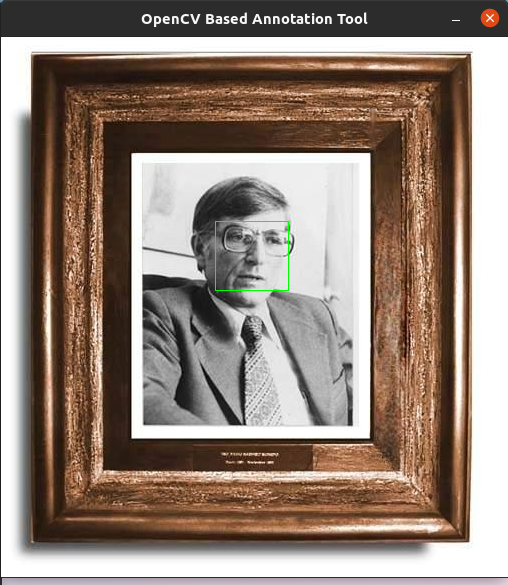
\includegraphics[scale=0.3]{faceAnnotation.png}
                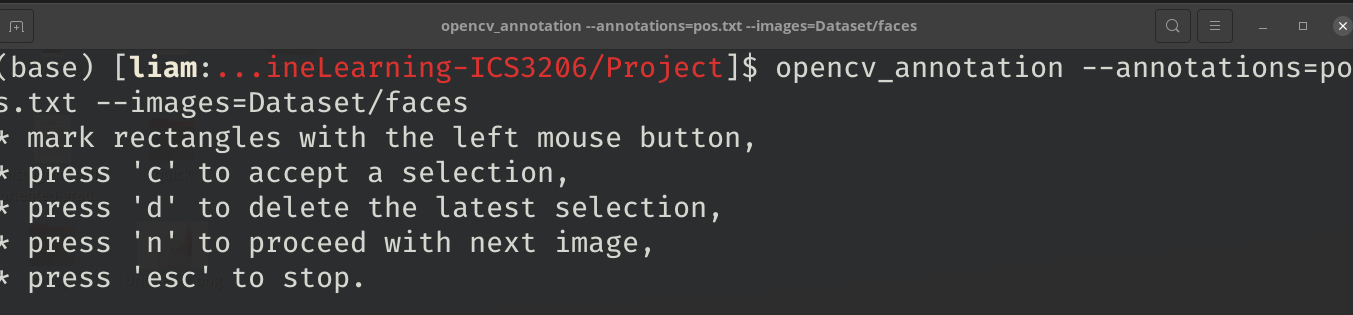
\includegraphics[scale=0.17]{terminalAnnotation.png}
                \caption{OpenCv Annotation Tool in progress}
                \label{annotationTool}
            \end{figure}

            \begin{figure}[H]
                \centering
                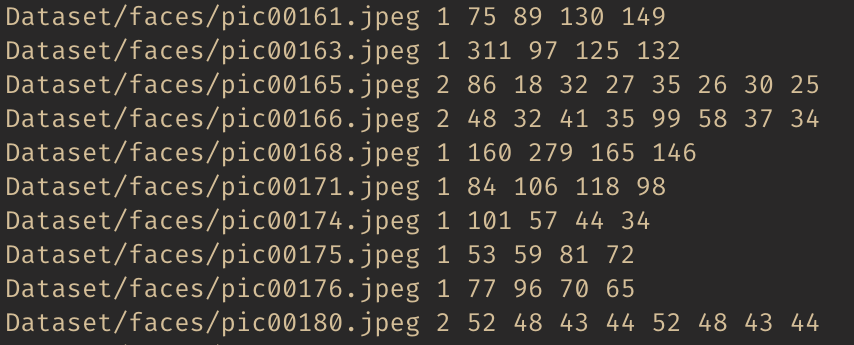
\includegraphics[scale=0.268]{postxt.png}
                \caption{Examples of the Positive Value File}
                \label{postxt}
            \end{figure}

        \subsubsection{Positive Vector File}
            A vector file generated from the positive values' text file is
            also required for cascade training which was generated using
            OpenCV's createSamples program.

    \subsection{Cascade Training}
        The next step is the boosted cascade of weak classifiers based
        on the positive and negative dataset prepared beforehand using
        OpenCV's train cascade function. Several models have been
        generated by changing the parameters' values to meet a good
        result. The evaluation section will show the model's results.
        The chosen model for this project which was generated by testing
        out different parameters contains the following parameters: 

            \begin{minted}[
                style=murphy,
            ]{shell}
$opencv_traincascade -data cascade 
-vec pos.vec -bg neg.txt -w 24 -h 24 
-numPos 800 -numNeg 425 -numStages 15
-precalcValBufSize 3000 -precalcIdxBufSize 
3000 -maxFalseAlarmRate 0.4
            \end{minted}

    \begin{itemize}
        \item \textbf{Number of stages: 15  (Started with 10 and
        increased to 15 for more accuracy but also keeping in mind
        overfitting)}
        \item \textbf{Maximum False Alarm Rate: 0.4}
        \item \textbf{Minimum hit Rate: 0.995}
        \item Number of positive samples: 800 (The Number of manualy annotated samples)
        \item Number of negative samples: 425
        \item Sample width: 24
        \item Sample weight: 24
        \item Number of unique features given window Size [24,24] : 162336
        \item Acceptance ratio break value: -1
        \item Stage type: BOOST
        \item Feature Type: HAAR
        \item Boost Type: GAB
        \item Weight Trim Rate: 0.95
        \item Max Depth: 1
        \item Max Weak Count: 100
        \item Mode: BASIC
    \end{itemize}


\subsection{Artefact 2}

    Artefact 2 The two downloaded models
    haarcascade\_frontalface\_default.xml, haarcascade\_eye.xml for
    the frontal face and eyes, respectively,  are tested using
    OpenCV's \textbf{cascadeClassifier} function. Check for the
    results and comparisons in the evaluation section.

\section{Evaluation and Results}

    \subsection{Artefact 1}
        The model's final stage contained \textbf{33 weak trees} with
        a \textbf{hit rate of 0.99625}, a \textbf{false alarm rate of
        0.383529} and a \textbf{negative acceptance ratio 425 :
        0.000470985}. In general, the model produces very good results
        as seen in figures \ref{one}, \ref{two} but produces some
        false faces when there are complicated backgrounds as seen in
        figure \ref{three}.

        \subsubsection{Some Good Results}

        \begin{figure}[H]
            \centering
            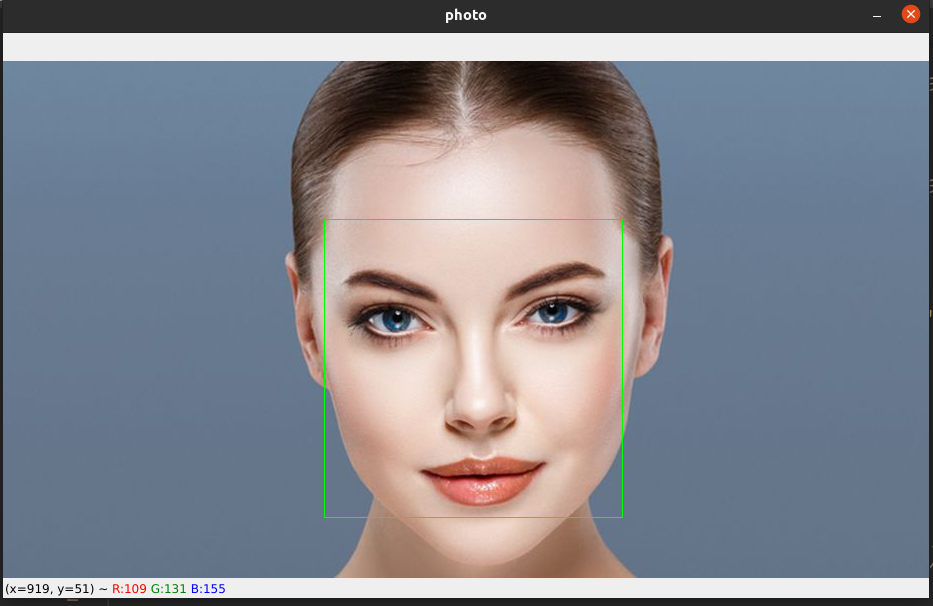
\includegraphics[scale=0.25]{goodImage2.png}
            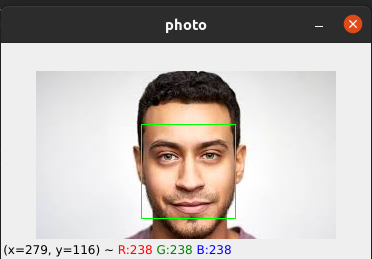
\includegraphics[scale=0.64]{goodResultPerson.png}
            \caption{Testing Results, (Images were not included in the dataset)}
            \label{one}
        \end{figure}

        \begin{figure}[H]
            \centering
            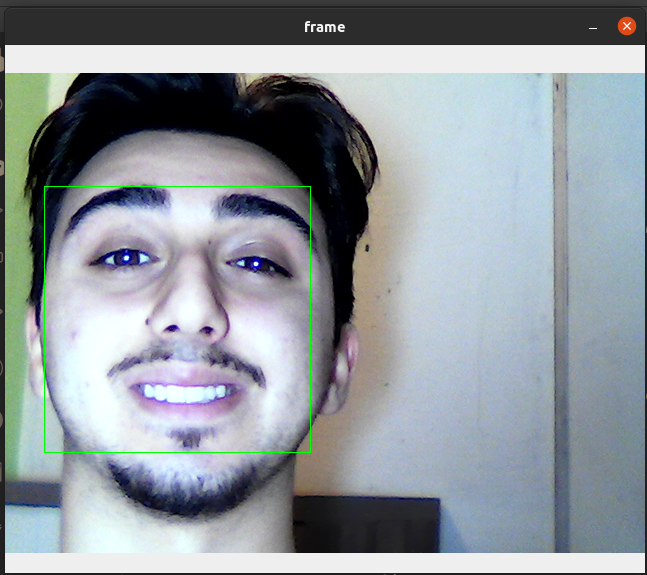
\includegraphics[scale=0.3]{goodResultWebcam.png}
            \caption{Webcam Result}
            \label{two}
        \end{figure}

        \begin{figure}[H]
            \centering
            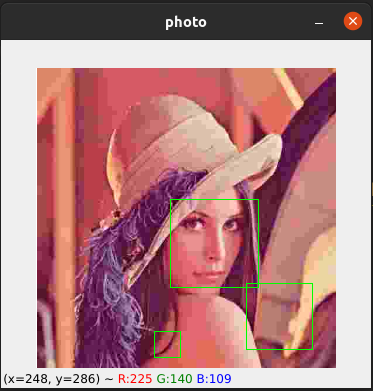
\includegraphics[scale=0.5]{goodImage1.png}
            \caption{Result with some Errors}
            \label{three}
        \end{figure}

        \pagebreak
        \subsubsection{Classification Metrics}
        some metrics when given 4 photos with a total of 24 faces.

        \begin{figure}[H]
            \centering
            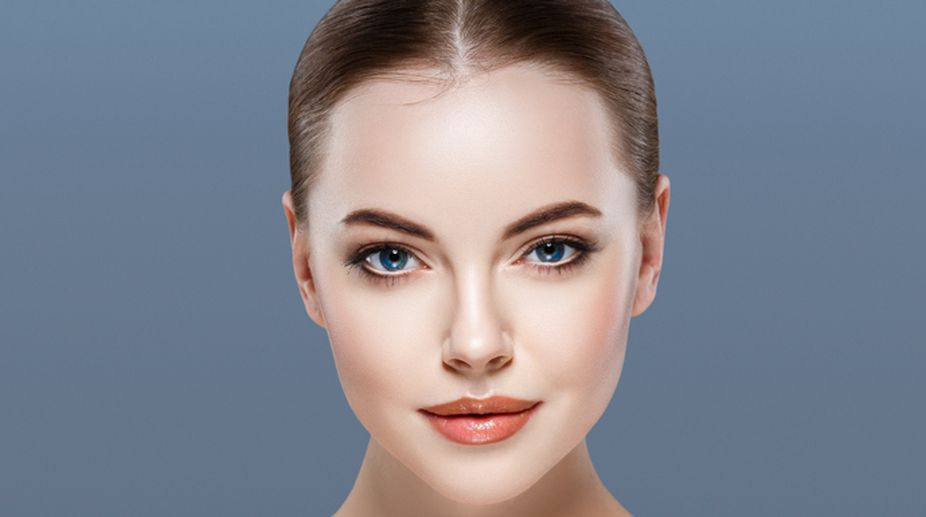
\includegraphics[scale=0.1]{testing/face1.jpg}
            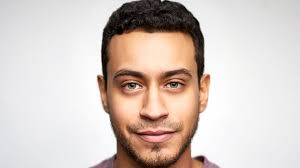
\includegraphics[scale=0.3]{testing/face2.jpeg}
            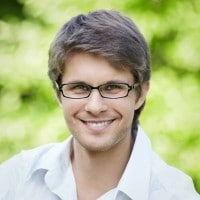
\includegraphics[scale=0.4]{testing/face4.jpg}
            
\includegraphics[scale=0.1]{testing/liverpool.jpg}
        \end{figure}

        \large{\textbf{Classification Accuracy}}
        \begin{equation}
            Accuracy=
            \frac{No \ of\ Good\ Predictions}{Total\ No\ of\ Predictions}
        \end{equation}

        \begin{center}
            27/20=0.64
        \end{center}

        \renewcommand\arraystretch{1.5}
        \setlength\tabcolsep{0pt}
        \begin{tabular}{c >{\bfseries}r @{\hspace{0.7em}}c @{\hspace{0.4em}}c @{\hspace{0.7em}}l}
        \multirow{10}{*}{\parbox{1.1cm}{\bfseries\raggedleft actual\\ value}} & 
            & \multicolumn{2}{c}{\bfseries Prediction outcome} & \\
        & & \bfseries p & \bfseries n & \bfseries total \\
        & p$'$ & \MyBox{26}{} & \MyBox{1}{} & P$'$ \\[2.4em]
        & n$'$ & \MyBox{13}{} & \MyBox{\footnotesize{All Background}}{\footnotesize{24x24\\segments}} & N$'$ \\
        & total & P & N &
        \end{tabular}

    \subsection{Artefact 2 results}

        \begin{figure}[H]
            \centering
            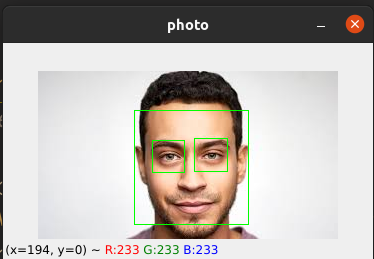
\includegraphics[scale=0.5]{art2Image3.png}
            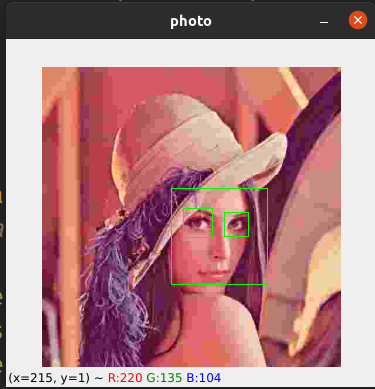
\includegraphics[scale=0.5]{art2Image2.png}
            \caption{Testing Results, (Images were not included in the dataset)}
            \label{one}
        \end{figure}

        \begin{figure}[H]
            \centering
            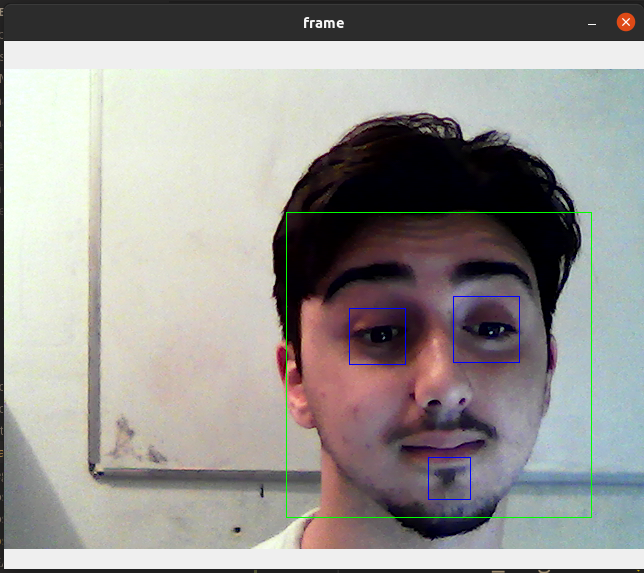
\includegraphics[scale=0.3]{art2Image5.png}
            \caption{Webcam Result}
            \label{two}
        \end{figure}
